\documentclass{article}
\title{Homework 1: The Knight's Tour}
\author{Kyle Hatfield kthvg5@mst.edu}
\date{\today}
\usepackage{amsmath}
\usepackage{algorithm}
\usepackage[noend]{algpseudocode}
\usepackage{graphicx}
\begin{document}
	\maketitle
	\begin{enumerate}
		\item The starting point for my algorithm was a Depth First Search (DFS). I designed a node data structure which contained a bool to note whether or not that node had been visited and a set of tuples representing the coordinates of the node's neighbors. A dictionary was used to store each of these nodes with a tuple containing their respective coordinates used at the key.
		
		Where this was efficient enough for a 6x6 board to be solved relatively quick (approximately 20 seconds), it was simply too slow for any larger tables. This became apparent when I let an 8x8 table run for almost ten hours before I gave up and canceled the operation. The reason behind this became apparent once I did the big O math on DFS. DFS is $O(b^d)$ where $b$ is the branching factor of the graph and $d$ is the depth of the goal state. $b$ at the worse case is equal to 8, and $d$ is equal the number of squares in the board, which in the case of an nxn table is $n^2$. So DFS of this application would be $O(8^{n^2})$. Yikes!
		
		However there is a Heuristic called Warnsdorf's rule which states that to find a open Knight's Tour in linear time, you simply pick the neighbor with the fewest neighbors for your next node. Applying this Heuristic to a DFS lowers the average branching factor $b$ substantially by removing the randomness inherent in DFS and giving it a good Heuristic to get most of the work done.
		
		\item There are three pieces of Python script in this tarball, dfs.py, wRule.py, and stack.py. dfs.py is a mock up of Depth First Search without Warnsdorf's Rule. It is just a referential piece of code that I wanted to keep in case I couldn't get the full version to work. wRule.py is the final code. stack.py contains a stack data structure I coded up over the summer so I would have it when I needed it.
		
		\item There are 26,534,728,821,064 tours.
	\end{enumerate}
	\begin{center}
		\begin{figure}[h]
			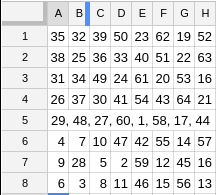
\includegraphics[width = \textwidth]{board}
			\caption {One possible solution to the knight's tour on an 8x8 board.}
		\end{figure}
	\end{center}
\end{document}